\begin{figure}[H]
    \centering
    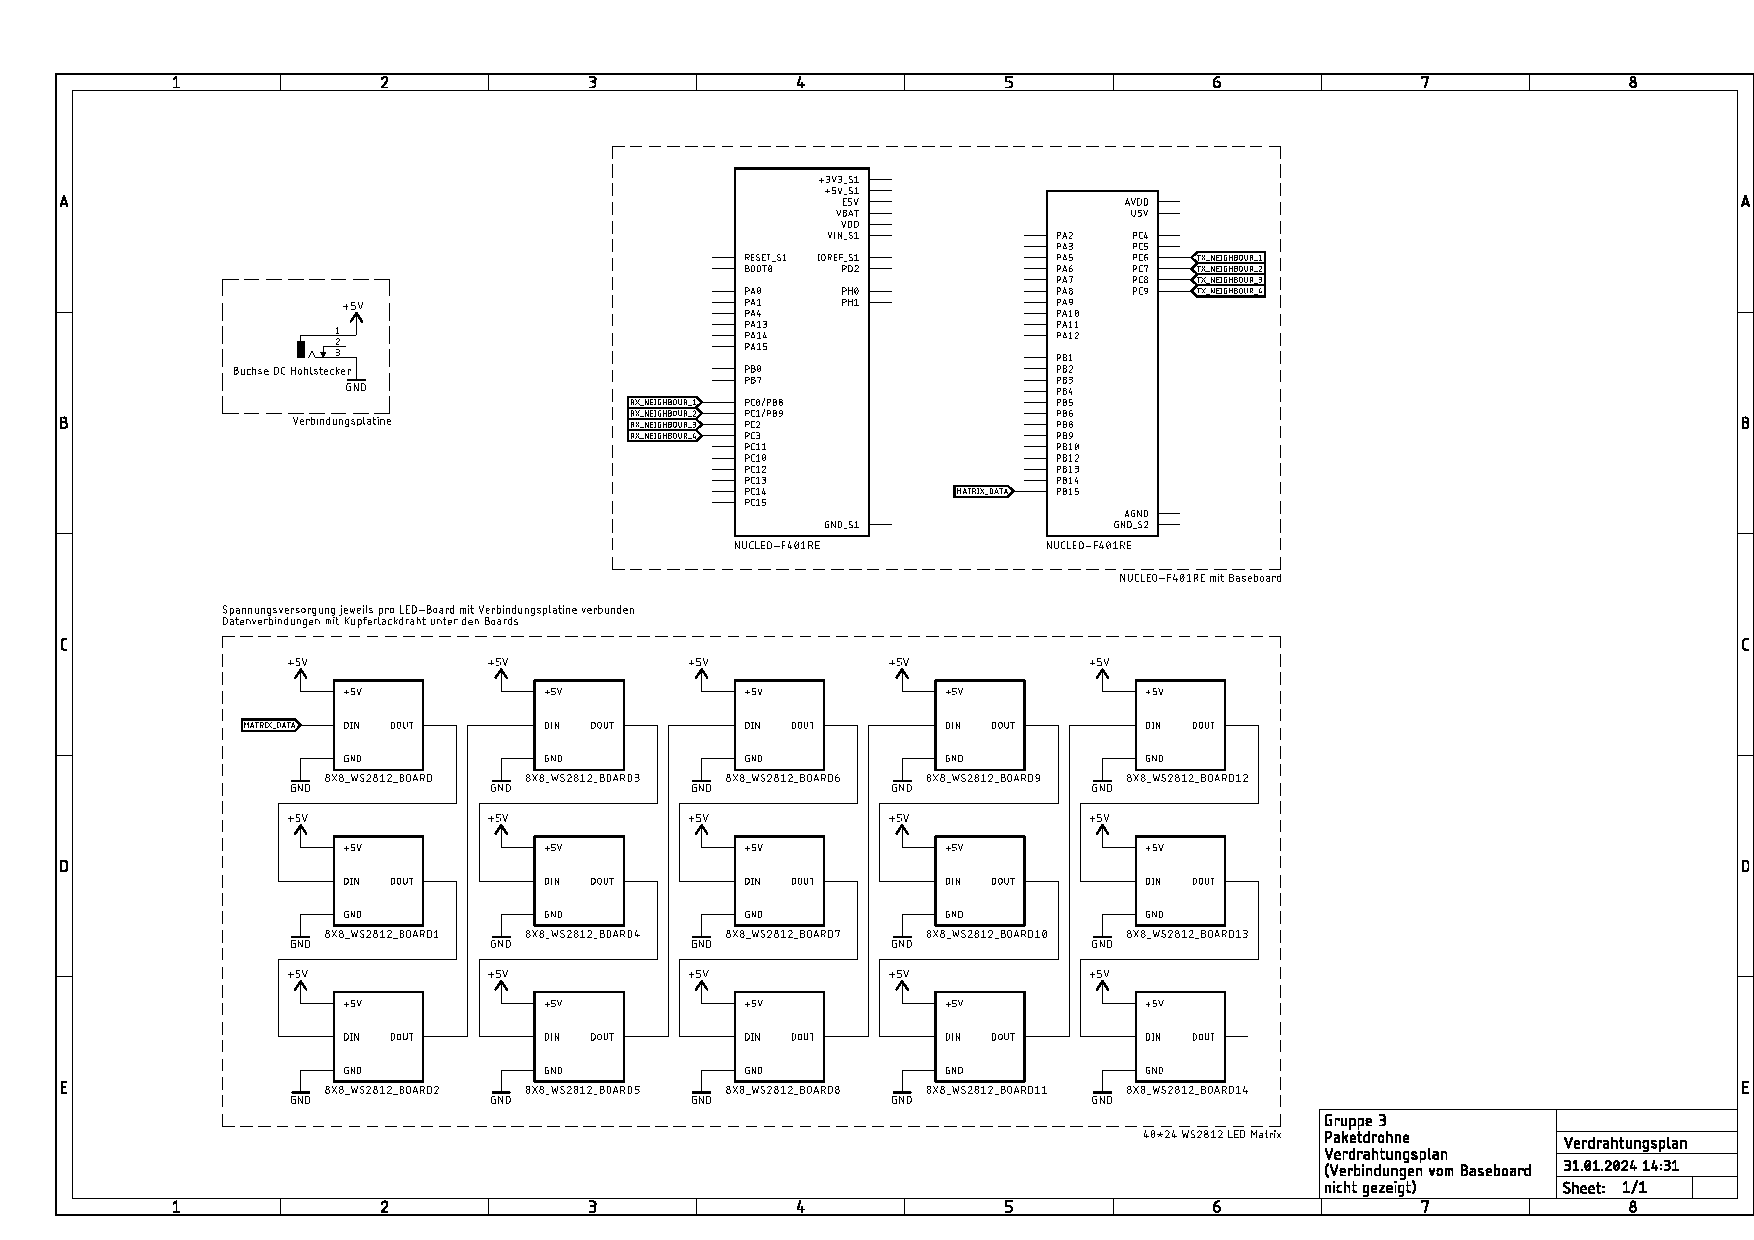
\includegraphics[angle=90,page=1,width=0.95\textwidth]{pdfs/Verdrahtungsplan.pdf} %angle = 270?
    \caption{Verdrahtungsplan}
    \label{fig:Verdrahtungsplan}
\end{figure}

\begin{figure}[H]
    \centering
    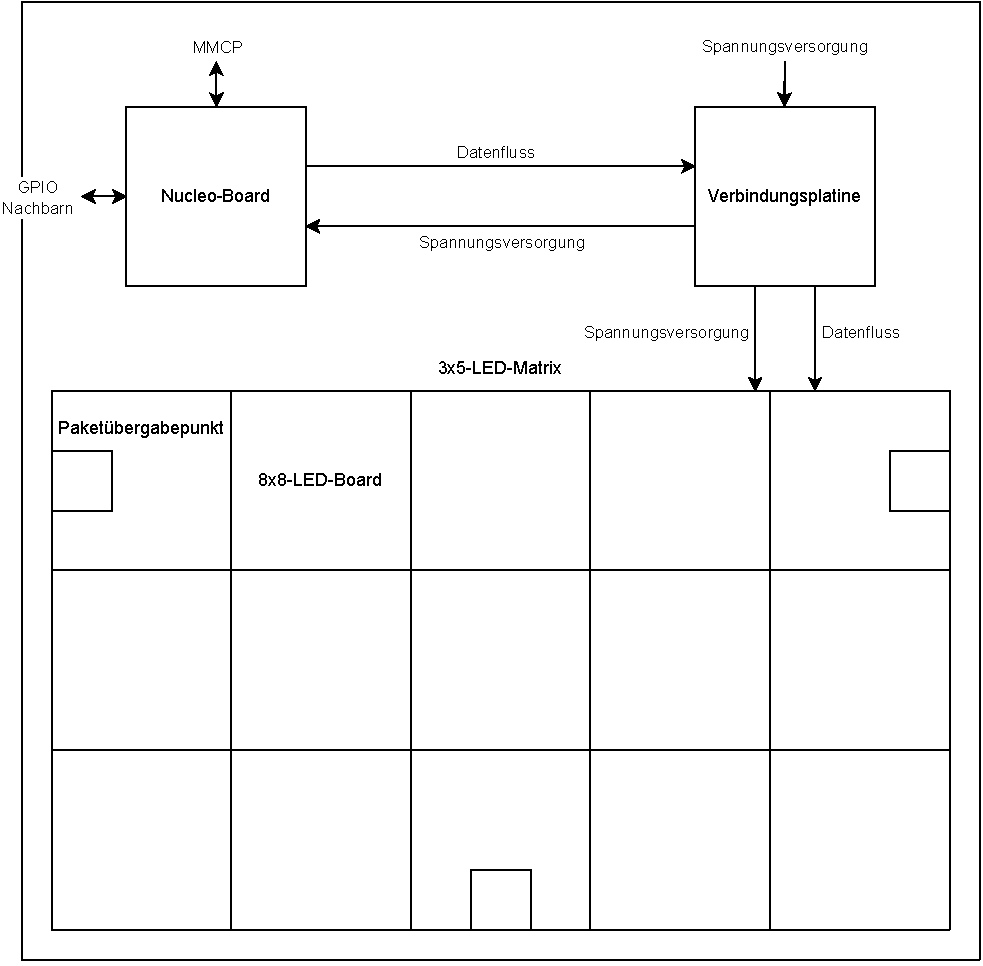
\includegraphics[width=0.75\textwidth]{pdfs/Konstruktionsskizze.pdf}
    \caption{Konstruktionsskizze}
    \label{fig:Konstruktionsskizze}
\end{figure}

\subsection{LED-Matrix}
Wie im Verdrahtungsplan (Abb. \ref{fig:Verdrahtungsplan}) gezeigt, besteht die 40x24 LED-Matrix aus 15 einzelnen Boards, welche jeweils 8x8 LEDs des Typs WS2812 besitzen. Alle LED-Boards sind mit Kupferlackdraht in Reihe geschaltet, sodass die gesamte Matrix mit einer Datenleitung angesteuert werden kann. Zudem hat jedes einzelne Board für die Spannungsversorgung zwei Leitungen zur Verbindungsplatine, um einem Spannungsfall in der Kette entgegenzuwirken.
\subsection{Nachbar-Pins}
Es können maximal 4 Nachbarn angeschlossen werden. Dafür gibt es für jeden Nachbar einen Empfangs- und einen Sendepin (\texttt{RX\_Neighbour\_x} bzw. \texttt{TX\_Neighbour\_x}). Die Empfangspins sind mit einem internen Pull-Down Widerstand konfiguriert. Um Interferenzen entgegenzuwirken, wurden alle Verbindungsleitungen mit einer nach Masse verbundenen Leitung umwickelt.